\documentclass[oribibl]{llncs}
\pagestyle{headings} %page numbers
\usepackage[T1]{fontenc}
\usepackage{hyperref}
\usepackage{graphicx}
\usepackage[utf8]{inputenc} 
\usepackage{todonotes}

\usepackage[font={footnotesize}]{caption}
\captionsetup[table]{skip=10pt}

\usepackage{subcaption}
\usepackage{amsmath}

\title{TERMES: Termite tracking in collaboration with Harvard University}
\author{Nikolaj Aaes \and Niklas Schalck Johansson \and Hildur Uffe Flemberg\\
\email{\{niaa, nsjo, hufl\}@itu.dk}}
\institute{IT University of Copenhagen \linebreak Rued Langgaards Vej 7  \linebreak DK-2300 Copenhagen S}
\date{December 2013}

\makeatletter
\renewcommand*\l@author[2]{}
\renewcommand*\l@title[2]{}
\makeatletter

\begin{document}
	
\graphicspath{{img/}} %default folder for image

\maketitle

\begin{abstract}
%!TEX root = Report.tex

10 linjer \\
problem stilling \\
evaluation \\
resultat \\

• State the problem - There is no existing software that allows tracking of termites. %using the HP plotter provided by harvard as well as being able to extract relevant statistics.\\
• Say why it’s an interesting problem - It will enable biologists to make better analyses based on more empricial data \\
• Say what your solution achieves - A way to control the plotter that tracks an ant/termite in real time and collects data that can be extracted as statistics\\
• Say what follows from your solution - While this is just a prototype (in a lab enviroment) it is a step towards making new and better field equipment for biologists along with corresponding software.\\

\label{abstract}
\keywords{Computer Vision, Image Processing, Termite Tracking, Biology, Computer Science.}

\end{abstract}

\setcounter{secnumdepth}{3}
\setcounter{tocdepth}{3}
\tableofcontents
\clearpage

%er koden kommenteret?
%læs igennem for specielle ord:
% Harvard University
% xy-plotter
% analyze/analyse 
% councillor / counsillor
% ant/termite

% lad hver af kapitlerne have en intro og en del-konklusion
% hæv abstraktion
% "vision based insekt tracking"
% 1,2,3 til et kapitel
% Camera feedback / robot control -> højt abstraktion
% rediger titler -> fortæl historie
% i tracking kan vi nævne at der findes andre ting -> her
% under hver "CV" teori vil vi gerne nævne hvad man opnår i forhold til projektet
% send inden/på torsdag

%!TEX root = Report.tex

\section{Introduction}

% Many species of termites, including ants, work in swarms to build structures that are many times larger than themselves. The fact that they do this in an efficient manner makes termites an interesting subject for study because we, as humans, can hope to learn from their techniques and apply them in a human context in construction of houses, bridges etc. Studying termite behavior, however, requires a lab environment facilitating appropriate hard- and software tools. \\
% 
% The goal of the Self-Organizing Systems Research Group (SOSRG) at Harvard University is to develop a swarm construction system in which robots cooperate to build 3D structures much larger than themselves. As of this writing, the system consists of simple robots that are able to move around and cooperate in and combining physical objects in order to build larger user defined pieces from high level descriptions. \\
% 
% This project is conducted at the IT University of Copenhagen (ITU) in the fall 2013 in cooperation with SOSRG. The goal of the project is to build software to interface with Harvard hardware in order to create a stand-alone environment for tracking and monitoring termites. Specifically, \\

This report is written at the IT University of Copenhagen (ITU) in the fall term of 2013 as a project supervised by Kasper Støy from ITU and with additional guidance from Kirstin Petersen from Harvard University. The project was developed from September 1st to December 16th 2013. The report is addressed to people interested in tracking ants or termites using image analysis. \\

%• General statement introducing the area; \\
%You can most likely start with the first paragraph from your project description and evolve it. - 

%• Explanation of the specific problem and why do we care about the problem. (MOTIVATON)\\

The Self-Organizing Systems Research Lab at Harvard University has created an autonomous robot for tracking African termites in a lab
environment but lacks the necessary software support. Working with and tracking these termites is cumbersome as they only thrive in
environments that resemble their native environment and only when they are together with other termites. Therefore automatic tracking of
specific termites is necessary, as tracking up until now has been done manually. \\

This project aims to develop software that is able to track both ants and termites in their native environment using a Hewlett-Packard provided by Harvard University. While it is already possible to communicate with the plotter using for instance Termite \cite{termite}, there is a need for software that integrates tracking, plotter communication, statistics and a graphical user interface. The end product is to be used by biologists and this software will lay the foundation to enable them to track ants/termites with more precision and with better and with better data being collected. Since biologists, who are the future end users of the product, would like to be able to stimulate the ants or termites with food or pheromones, we need a non-stationary part which is exactly what the plotter provides (the plotter arm). \\

%• Explanation of your solution, and how it improves on the work by others. Relation to related work can be very brief, given that you have a separate extensive section devoted to this. \\
A team at Harvard University previously experimented \todo{kan vi få en ref til deres projekt?}with using the plotter to track a single ant on a white background with some success. While the details of this effort were unknown to us we decided to start this project from scracth. Since this team had some success with their approach we use their hardware setup as a starting point for this project. The focus of the project is mainly on the development of the software and the selected hardware has a secondary role. \\

\begin{figure}
        \centering
        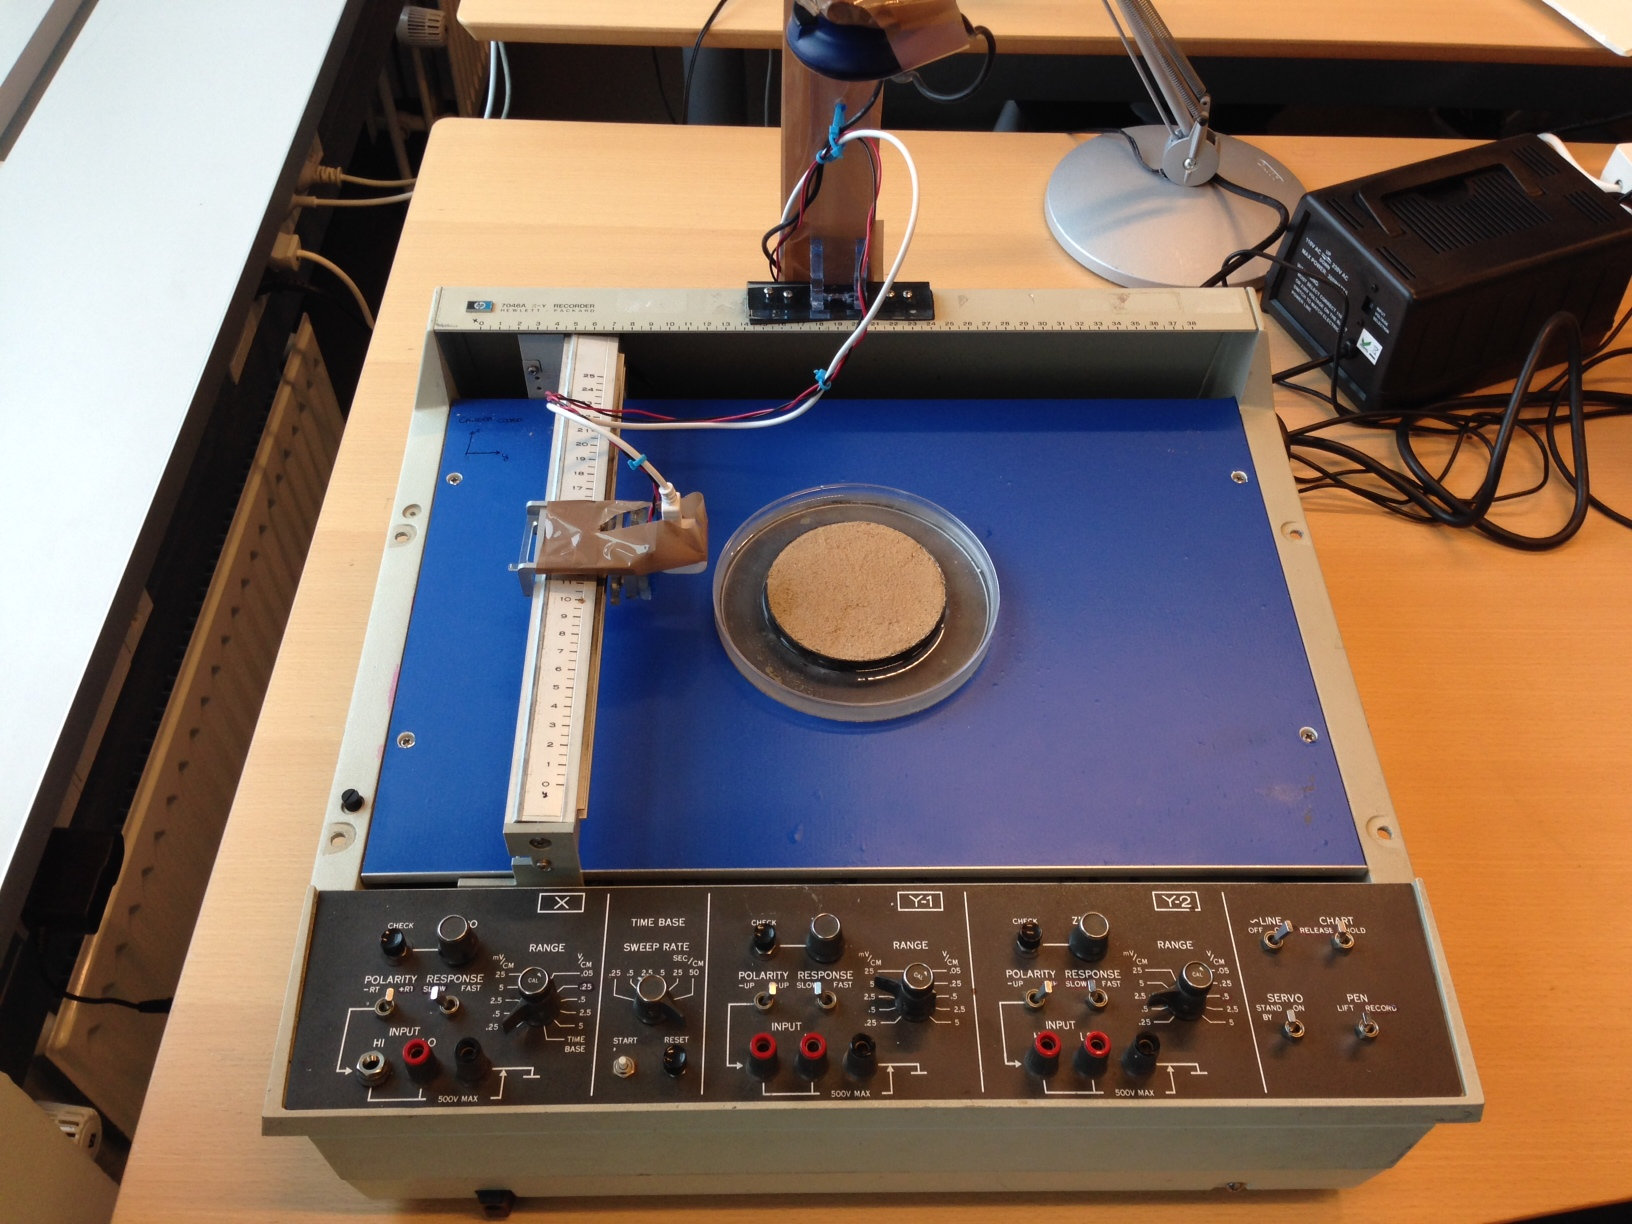
\includegraphics[scale=0.125]{img/plotter}
        \caption{Plotter with mobile camera, overhead camera and control panel}
        \label{fig:plotter}
\end{figure}

%• A hint on how the solution was evaluated and what was the outcome of this evaluation. \\
Since tracking of ants is very hard to test systematically we have chosen to evaluate it by describing in which cases we expect the tracking to work as intended and in which cases we expect it not to. The results show that tracking of ants are both possible and satisfactory but still have cases where the it will fail. Both the results and possible improvements can be found in Section \ref{testing}.\\

The project was undertaken as a substitute for the "Global Software Development" course at ITU and therefore has additional emphasis on the international collaboration and development process. Section \ref{process} will describe the collaboration tools used as well as evaluate the overall process. \\ 

%A summary (a “map”) of how the paper is organized.\\
This report assumes that the reader has a basic knowledge of mathematics but any prior knowledge about computer vision is not required. We will first describe the requirements and scope of the project and the image analysis theory we either considered or used in the project. Then we will describe how we interacted with the XY-plotter and how we combined this with the tracking. Lastly will we describe the tests, analyze the results and conclude the project.





%!TEX root = Report.tex

\subsection{Project Proposal}

%The Self-Organizing System Research Lab on Harvard has created a autonomous robot for tracking African termites in a lab environment. Working with and tracking these termites is cumbersome as they only thrive in environments that resemble their native environment and only when they are together with other termites. Therefore automatic tracking of specific termites is necessary, as tracking up until now has been done manually. Hardware has been created to handle this, however it lacks proper software support. \\

The purpose of this project is to develop software, such that the provided hardware can be used to track ants or termites, extract relevant statistics, as well as providing basic user input to the robot tracker. \\

There are three parts in this project:  

\begin{enumerate}
\item Tracking ants using a low resolution camera. In order to track an ant, it is necessary to be able to determine its position and move the camera to its new position using image analysis on the camera output. 

\item Interact with the plotter and update the camera's position with the result from the tracking software. 

\item Design and develop a user interface that can be used to retrieve statistical data from the tracking.  
\end{enumerate}

\section{Vision based insect tracking}

%!TEX root = Report.tex

\section{Background}

%Projektet er erstatning for GSD hvad betyder det for os? (ved ikke om det skal med)
%Hvilket udstyr havde vi at arbejde med?
%Umiddlebart ville vi gerne have logic code i C++ og GUI i Java så vidt muligt. Hvilke fordele giver det os? hvorfor?
%Hvad for nogen myrer havde vi og var der nogen udfordringer her? (tænk: hvis jeg skal gøre det igen, hvad skal jeg så huske om myrer)
%Hvordan var det med at male myrerne?

This project was undertaken as a substitute for the "Global Software Development" course at ITU and therefore has additional emphasis on the international collaboration and developement process. Section \ref{process} Process will describe the tools used as well as evaluate the overall process. \\ 

Our councillor at Harvard wanted the tracking and the interfacing with the tracking device to be implemented in C++ to make it easier for further developement. The graphical user interface was not restricted when choosing programming langauge and we ended up using C\# and Windows Forms to implement it.

As mentioned in the project proposal the project was divided into three parts. The first part of the project was to be able to track termites. Since african termites are hard to come by and transport we settled for giant ants (Camponotus Ligniperdus), which are the largest ants found in Denmark \cite{fogn}, instead. While these are not as big as the termites, they behave in a similar way and the solution should be able to easily adapt to the termites. In the first part we started by implementing the tracking on a video. We received a video from Harvard of a single ant running around in a petri dish with a white background. The ant itself was painted red and green to make tracking easier. This was the simplest setup we could think of and acted as a good starting point. By recommendation we decided to use the OpenCV \cite{opencv} framework to implement our tracking. We will return to this framework in Section \ref{framework} Framework. \\

The second part of the project interacting with our tracking device and conform the tracking code to work with the device. We received a Hewlett-Packard 7046a XY-plotter by mail from our councillor at Harvard. Additionally we received a small ant farm, containing one queen and seven worker ants (no soldier ants), via mail and we bought some brushes and acryllic paint for the ants. The ants did not proliferate during the project. While we discussed using infrared paint or fluorescend paint, both these ideas were discarded because both types of paint contains compounds that the termites and ants really like which makes them eat the painted ant. Along with the plotter we also received a small circuit board that plugged into the serial port of the plotter and had a USB cabel for us to communicate with it. Lastly the package contained a collection of petri dishes for us to use. \\

In this part we had to paint the ants with the paint we bought and we want to give some friendly advice to anyone who wants to do any projects involving ants. If you put them 2-4 minutes in the freezer they become very docile and much easier to paint without harming the ants. When they are taken out they act completely normal after 2-3 minutes. The ants also had a tendency to crawl up the sides of the petri dish. We were recommended to try putting teflon tape (should be really slippery) on the sides without any luck. We were also recommended to try mineral oil but we were unable to get any. Our solution was to place a small petri dish in a bigger petri dish and fill the gap with water. The ants would quickly discover that there was water surronding them which prevented them from escaping the small petri dish. \\

The third part of the project involved constructing the graphical user interface, hooking it up to the tracking code and extracting statistics.  \\

TODO: beskriv third part. Skriv at myrer godt kan svømme! plus de problemer vi havde med at holde myrene inden for petri skålen.  

\subsection{Assumptions}

TODO

\subsection{Scope}

%Kun test i et lab environment
%test på myrer, regner med at det kan generaliseres til termitter (andre størrelser)
%Kun test med de farver maling vi har
%Kun test med denne plotter
%Kontrollerede lysforhold
%Tracker kun een myre ad gangen

While the project lays the foundation for a fully useable field solution we have chosen to narrow our scope to the essential functionality. This also means that the project was designed and tested in a controlled lab environment where factors such as lighting, wind etc. are constant. \\

Because actual termites were out our reach and that our councillor at Harvard recommended it, we did all of our testing with normal ants instead of termites. We are confident that only minor adjustments are necesarry to make the solution work with termites since the main difference is the size. \\

Painting the ants in different colors can have some impact in the quality of the tracking. As a rule of thumb it is easier to track colors that contrast the background the most. In this project we chose to paint the ants white and bright green. We did not try any other colors because we found these to have a high degree of contrast which were sufficient. \\

As the HP 7046a plotter was the only hardware available to us we have restricted the project to only include this type of plotter. One could potentially gain better results with a plotter with a finer granularity in coordinates and smoother movement. The cameras supplied with the plotter was also the only cameras available to us and we have therefore also restricted the project to only include these cameras. While one could use higher resolution cameras to obtain a better result, the weight of the camera is also important for the smoothness of the movement of the plotter and must be carefully considered.\\

While it could be intereseting to track several ants we have chosen to focus on tracking a single ant in this project due to time restrictions. However, we do not believe that there are any technical barriers against this and would simply require more time to implement.\\

TODO: \\
fortæl om hvordan vi IKKE tester

\subsection{Requirements}

\subsubsection{Mandatory requirements}
The mandatory requirements of the project are listed below and must be fulfilled for the project to be considered a success.

\begin{enumerate}
    \item Tracking of ants and/or termites using a low resolution camera using C/C++.
    \item The ability to adjust the tracking parameteres before and during the tracking.
    \item Moving the tracking hardware in corresponding to the tracking.
	\item A graphical user interface containing two modes:
    \item - Calibration mode. Must contain a direct feed from the lower camera, a proccessed feed and sliders to adjust the processing.
    \item - Tracking mode. Must contain a direct feed from the lower camera, a direct feed from the overhead camera and statistics.
    \item The ability to collect the following statistics:
    \item - The route of the ant/termite over time. 
    \item - Heatmap of where in the petri dish the ant stay.
    \item The ability to save the collected statistics.
\end{enumerate}

\subsubsection{Optional requirements}
The optional requirements are the so called "nice-to-have requirements". They are not mandatory for the project but features that could be desirable to implement if the time and resources permits it.

\begin{enumerate}
	\item An additional third mode in the graphical user interface Bias mode: adds the ability to select a certain point which the plotter will try to lure the termites towards using food or pheromones.
    \item The ability to choose certain areas which should be avoided during the tracking.
    \item Collection of these additional statistics:
    \item - Average speed of the ant/termite.
    \item - The amount of ants/termites meet during the tracking. A way to adjust what defines a meeting.
    \item - The amount of time between each meeting. A way to adjust when a meeting starts and ends.
    \item - The duration of each meeting.
    \item - The area of the petri dish covered by the ant/termite. A way to adjust how much area is covered by an ant/termite when stationary (also known as "headsize").
    \item - How much area is covered over time.
    \item - Mean free path (the amount of time between each "stay").
\end{enumerate}




%!TEX root = Report.tex

\subsection{Tracking}
\label{tracking}
As mentioned in the project proposal the project was divided into three parts. The first part of the project was to be able to track termites. Since african termites are hard to come by and transport we settled for giant ants (Camponotus Ligniperdus), which are the largest ants found in Denmark \cite{fogn}, instead. While these are not as big as the termites, they behave in a similar way and the solution should be able to easily adapt to the termites. In the first part we started by implementing the tracking on a video. We received a video from Harvard of a single ant running around in a petri dish with a white background. The ant itself was painted red and green to make tracking easier. This was the simplest setup we could think of and acted as a good starting point. By recommendation we decided to use the OpenCV \cite{opencv} framework to implement our tracking. We will return to this framework in Section \ref{framework} Framework. \\

This chapter is divided into three subparts. First we will introduce the reader to different image processesing techniques, and their uses. Following this we will introduce the reader to a framework that supports these techniques, and finish off describing the implemented solution and design choices.

% Gå ud fra at dette afsnit ikke har noget video input fra et kamera. Integration med kameraet kommer senere.
% 
% Teori først - hvilken slags image manipulation har vi brugt? hvad var alternativerne?
% Så framework - vi bruger OpenCV, why? hvad giver det os? hvad er drawbacks?
% så implementation - Hvad har vi implementeret? Hvordan var performance? hvad var vores alternativer? har vi eksperiementeret med nogen af de andre muligheder?
% 
% Image Segmentation - hvad giver det os/hvorfor er det smart?
% Thresholding
% Dilating
% Eroding
% Background detection and why we can't use it
% Alternatives and why we don't use them

\subsubsection{Theory} \mbox{}\par
\todo{Rewrite chapter a bit - make it self contained. Keep writing WHY this is important and interesting to read and how it will help track ants.}
This section will provide information about five common image processing techniques; thresholding, dilating and eroding, contrast, image segmentation and background filtering. The description of each technique will be backed up by examples. We will also use the \textit{ternary if} statement notation in this section which looks like the one shown in Equation \ref{eq:notation}.

\begin{equation}
value = {Boolean\mbox{-}Condition} ? {True\mbox{-}Evaluation}: {False\mbox{-}Evaluation}
\label{eq:notation}
\end{equation}

It works just like you would expect from many programming languages. It is also known as an inline \textit{if-statement}. \\

\noindent \textbf{Thresholding} \par
Thresholding is an image processing technique used to make a final decision about each pixel in an image. Either a pixel value is one that we are interested in or it is not. This is usually done by assigning a specific pixel value to the pixel we want, and another to those that we do not want. In general we compare the \textit{i}th pixel of the source image, \textit{src}, to the threshold value, \textit{T}, and saves the result in a destination image, \textit{dst}. For instance, to create a binary image where we are interested in all pixels above the threshold \textit{T}, the equation would look like the one shown in Equation \ref{eq:binarythresholding},

\begin{equation}
dst_i = src_i \geq T ? 255: 0
\label{eq:binarythresholding}
\end{equation}

Most threshold operations are applied on grayscale images, where all pixel values range between 0 (black) and 255 (white). Sometimes these values are normalized to range between 0 and 1 instead. However for the rest of this report we will assume that grayscale images use the former convention. Soon we will argue how thresholding can be expanded to also cover thresholding an RGB image. Figure \ref{fig:threshold_example} show an example of applying threshold to a grayscale image.

\begin{figure}
        \centering
        \begin{subfigure}[b]{0.3\textwidth}
                
\includegraphics[scale = 0.2]{img/globe}
                \caption{Grayscale image}
        \end{subfigure}
		\quad
        \begin{subfigure}[b]{0.3\textwidth}
                
\includegraphics[scale = 0.2]{img/post_threshold}
                \caption{Thresholded image}
        \end{subfigure}
		\caption{An example of applying a threshold on a grayscale image. This example use the threshold value \textit{T} = 200}
		\label{fig:threshold_example}
\end{figure}

Now what happens if what you are interested in is a color? To use standard thresholding we first need to convert it to a grayscale image. However doing so might result in an image that have lost important information as can be seen in figure \ref{fig:RGB2GRAY}. Unless you want to find the red color, you have no way of differentiating the blue and green color.

\begin{figure}
        \centering
        \begin{subfigure}[b]{0.3\textwidth}
                
\includegraphics[scale=0.5]{img/RGB}
                \caption{RGB image}
        \end{subfigure}
		\quad
        \begin{subfigure}[b]{0.3\textwidth}
                
\includegraphics[scale=0.5]{img/GrayRGB}
                \caption{Grayscale image}
        \end{subfigure}
		\caption{Example of grayscaling a color image}
		\label{fig:RGB2GRAY}
\end{figure}

A step in the right direction would be to define the threshold value \textit{T} as a scalar consisting of three values - one for each color channel. We will denote this threshold scalar as \textit{S} and define it as shown in Equation \ref{eq:thresholdscalar}.

\begin{equation}
S =  
\begin{pmatrix}
  S_{R}\\
  S_{G}\\
  S_{B}\\
\end{pmatrix}
\label{eq:thresholdscalar}
\end{equation}

To apply it to an RGB image we need to change Equation \ref{eq:binarythresholding} to the one shown in Equation \ref{eq:threshold_RGB}.

\begin{equation}
{dst_i} = {src_i}_R \geq S_R \wedge {src_i}_G \geq S_G \wedge {src_i}_B \geq S_B? 255: 0
\label{eq:threshold_RGB}
\end{equation}

Trying it out makes it much easier to differentiate between colors. In Figure \ref{fig:RGB_Thresh} a threshold attemp using this method directly on the RGB image is shown.

\begin{figure}
        \centering
        \begin{subfigure}[b]{0.3\textwidth}
                
\includegraphics[scale=0.5]{img/RGB}
                \caption{RGB image}
        \end{subfigure}
		\quad
        \begin{subfigure}[b]{0.3\textwidth}
                
\includegraphics[scale=0.5]{img/RGBThresh}
                \caption{Thresholded image}
        \end{subfigure}
		\caption{Example of thresholding a color image with Equation \ref{eq:threshold_RGB} using the scalar \textit{S}=(0,100,0)}
		\label{fig:RGB_Thresh}
\end{figure}

However one issue remains - what if you want to find a color among similar colors? The problem is illustrated in Figure \ref{fig:green_fail} using the same scalar as in Figure \ref{fig:RGB_Thresh}

\begin{figure}
        \centering
        \begin{subfigure}[b]{0.3\textwidth}
                
\includegraphics[scale=0.5]{img/green}
                \caption{RGB image}
        \end{subfigure}
		\quad
        \begin{subfigure}[b]{0.3\textwidth}
                
\includegraphics[scale=0.5]{img/simpleRGBThresh}
                \caption{Thresholded image}
        \end{subfigure}
		\caption{Example of thresholding a color image with Equation \ref{eq:threshold_RGB} using the scalar \textit{S}=(0,100,0). Unlike before the result is unsatisfactory.}
		\label{fig:green_fail}
\end{figure}

The solution is to specify a \textit{range} of acceptable values instead of just a threshold. We will specify two scalars; S Upper, \textit{SU}, and S Lower, \textit{SL}.

\begin{equation}
SL =  
\begin{pmatrix}
  SL_{R}\\
  SL_{G}\\
  SL_{B}\\
\end{pmatrix}
\label{eq:thresholdlower}
\end{equation}

\begin{equation}
SU =  
\begin{pmatrix}
  SU_{R}\\
  SU_{G}\\
  SU_{B}\\
\end{pmatrix}
\label{eq:thresholdupper}
\end{equation}

We will use the definitions in Equations \ref{eq:thresholdlower} and \ref{eq:thresholdupper} to update Equation \ref{eq:threshold_RGB}. The changes can be seen in Equation \ref{eq:threshold_range}.

\begin{equation}
{dst_i} = SU_R \geq {src_i}_R \geq SL_R \wedge SU_G \geq {src_i}_G \geq SL_G \wedge SU_B \geq {src_i}_B \geq SL_B? 255: 0
\label{eq:threshold_range}
\end{equation}

Using a range to specify a color instead will yield a much more satisfactory result as shown in Figure \ref{fig:green_final}. \\

\begin{figure}
        \centering
        \begin{subfigure}[b]{0.3\textwidth}
                
\includegraphics[scale=0.5]{img/green}
                \caption{RGB image}
        \end{subfigure}
		\quad
        \begin{subfigure}[b]{0.3\textwidth}
                
\includegraphics[scale=0.5]{img/finalthresh}
                \caption{Thresholded image}
        \end{subfigure}
		\caption{Example of thresholding a color image with Equation \ref{eq:threshold_range} using the range \textit{SL}=(0,100,0) and \textit{SU}=(1,150,10). We have sucessfully located the dark green color area.}
		\label{fig:green_final}
\end{figure}

\newpage

\noindent \textbf{Dilation and Erosion} \par
% Forklar at vi har en kernel, B, med størrelsen s, der bliver anvendt på hver pixel, p, i et billede A.
% Angiv at dilating finder local optima, og at eroding finder local minima.
% Angiv at de her metoder bliver brugt EFTER thresholding for at "rense" billedet. \\

The basic concepts of \textit{morphological transformations} are \textit{dilation} and \textit{erosion}. These concepts are mostly used to remove noice, isolating individual elements or joining disparate elements in an image. These transformations are applied to either grayscale or binary image, and are often used to clean up an image after thresholding to make analysing the image easier. The way both erosion and dilation are applied to an image is by defining a kernel, denoted \textit{B}, that will be applied to an image (or part of an image), denoted \textit{A}. The kernel can be any shape or size, however it is often a square where the sides are uneven, e.g. 3x3, 5x5, 7x7 and so on. A kernel has an \textit{anchorpoint}, which is the pixel in A that erosion or dilation are applied on, and the result is stored in the corresponding point in the destination image, \textit{dst(i.j)}. Figure \ref{fig:kernel_ed} shows an example of a kernel and its anchorpoint in the center. \\

\begin{figure}[ht!]
  \centering
    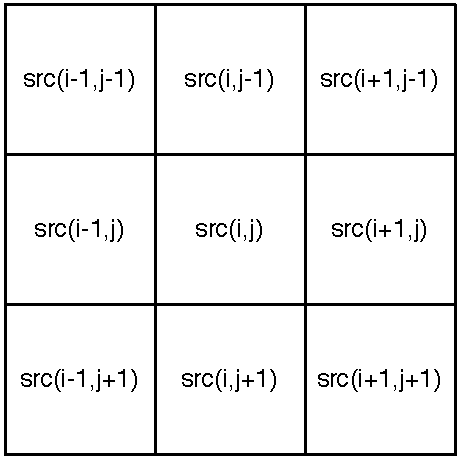
\includegraphics[scale=0.50]{img/Kernel_ED.pdf}
  \caption{Given a pixel, src(i.j) the kernel covers the neighbouring pixels. Shown here is a 3x3 kernel.}
  \label{fig:kernel_ed}
\end{figure}

When transforming an image using dilation, whenever the kernel is applied to a new anchorpoint, the \textit{local optima} is used. When eroding an image the \textit{local minima} is used. Naturally, compared to the original image, bright areas are expanded when dilating, and dark areas are expanded when eroding. However one cannot say that e.g. eroding removes noice and dilating does not. It depends on the image which the transformation is applied on. Figure \ref{fig:sample_kernel} shows an example of pixels used to determine the outcome of the anchorpoint in the destination image. \\

\begin{figure}[ht!]
  \centering
    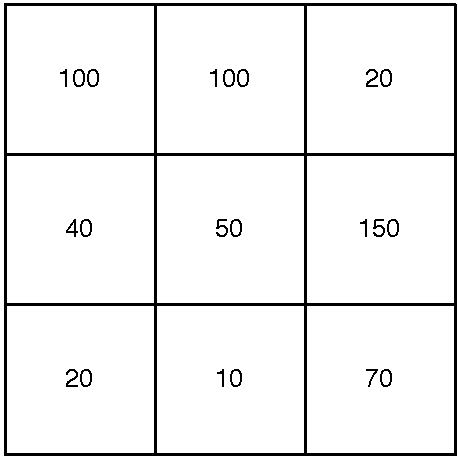
\includegraphics[scale=0.50]{img/sample_kernel.pdf}
  \caption{An example of a kernel within a source image, src. The value assigned to the destination image, dst(i,j), is 10 if erosion is chosen, else 150 if dilation is chosen.}
  \label{fig:sample_kernel}
\end{figure}

An example of how this applies to a real image is shown in Figure \ref{fig:erodedilate}. It is clear from this example how differently erosion and dilation affects an image.\\

\begin{figure}[!ht]
        \centering
        \begin{subfigure}[b]{0.3\textwidth}
                
\includegraphics[scale = 0.2]{img/globe}
                \caption{Grayscale image}
        \end{subfigure}
		\quad
        \begin{subfigure}[b]{0.3\textwidth}
                
\includegraphics[scale = 0.2]{img/erode}
                \caption{Eroded image}
        \end{subfigure}
		\quad
        \begin{subfigure}[b]{0.3\textwidth}
                
\includegraphics[scale = 0.2]{img/dilate}
                \caption{Dilated image}
        \end{subfigure}
		\caption{Eroding and dilating an image. It is clear that eroding expands dark areas and dilate expands bright areas. This example uses a 7x7 kernel.}
		\label{fig:erodedilate}
\end{figure}

Unlike thresholding we cannot apply erosion or dilation to RGB images due to the nature of \textit{RGB} values. Imagine the clear colors, red (255,0,0), green (0,255,0) and blue(0,0,255) - how can we argue which color is \textit{greater} or \textit{smaller} than the other? We cannot. We can with grayscale and binary images since we can safely say that the pixel value 150 is smaller than 255, and 0 is smaller than 1. We cannot for color images. \\

\noindent \textbf{Contrast and Brightness} \par
Where dilation and erosion sought to expand either dark or bright areas, contrast and brightness seek to increase the overall brightness or darkness of an image or the absolute difference between dark and bright pixels. To increase the absolute difference difference between two pixels, or \textit{increasing the contrast of the image}, each pixel in an image is multiplied with the same scalar, denoted $\alpha$. Since images are basically matrices this method is equal to \textit{scalar multiplication} shown in Equation \ref{eq:matrix_mul}.

\begin{equation}
\alpha \times 
\setlength{\arraycolsep}{5pt}
 \begin{bmatrix}
  a & b & c \\
  d & e & f \\
  g & h & i \\
 \end{bmatrix} =
 \setlength{\arraycolsep}{5pt} 
 \begin{bmatrix}
  \alpha \times a & \alpha \times b & \alpha \times c \\
  \alpha \times d & \alpha \times e & \alpha \times f \\
  \alpha \times g & \alpha \times h & \alpha \times i \\
 \end{bmatrix}
 \label{eq:matrix_mul}
\end{equation}

To increase the brightness each pixel is added with a scalar, denoted $\beta$ instead. This way the absolute difference between each pixel is kept, however all pixels get darker or brighter depending on the scalar. Similar to contrast this operation is equal to \textit{scalar addition} as shown in Equation \ref{eq:matrix_add}. To make the pixels brighter a positive scalar is used, to make it darker a negative scalar is used. Figure \ref{fig:bright_contrast} shows the result of contrasting and increasing the brightness of an image. Contrast and brightness are used to make dark, bright and diffuse images easier to analyse. \\

\begin{equation}
\beta + 
\setlength{\arraycolsep}{5pt}
 \begin{bmatrix}
  a & b & c \\
  d & e & f \\
  g & h & i \\
 \end{bmatrix} =
 \setlength{\arraycolsep}{5pt} 
 \begin{bmatrix}
  \beta + a & \beta + b & \beta + c \\
  \beta + d & \beta + e & \beta + f \\
  \beta + g & \beta + h & \beta + i \\
 \end{bmatrix}
 \label{eq:matrix_add}
\end{equation}

\begin{figure}
        \centering
        \begin{subfigure}[b]{0.3\textwidth}
                
\includegraphics[scale = 0.2]{img/colorGlobe}
                \caption{Source image}
        \end{subfigure}
		\quad
        \begin{subfigure}[b]{0.3\textwidth}
                
\includegraphics[scale = 0.2]{img/globeBright}
                \caption{Brightened image}
        \end{subfigure}
        \begin{subfigure}[b]{0.3\textwidth}
                
\includegraphics[scale = 0.2]{img/globeContrast}
                \caption{Contrasted image}
        \end{subfigure}
		\caption{Example of increasing the contrast and brigtness of an image. For this example $\alpha = 5$ and $\beta = 100$}
		\label{fig:bright_contrast}
\end{figure}

\noindent \textbf{Image Segmentation} \par
Image segmentation is the processing of partitioning all the pixels in an image into \textit{S} segments (or superpixels). The goal is to simplify or change the representation of an image such that it is easier to analyse. It is mostly used to locate objects that consist of a range of similar colors, that is combined into a single colored object after segmentation, thus making it easier to find. Image segmentation is therefore the process of assigning a label to a pixel, such that such that pixels with the same label share certain visual characteristics. The result of image segmentation is a set of segments that covers the entire image. Thresholding, as described earlier, is the simplest method of segmenting an image. \\

One of the most common algorithms to segment images is the \textit{k-means} algorithm. K-means is a \textit{clustering algorithm} often used in \textit{datamining} in the \textit{unsupervised learning} category. What k-means basically does it to take a set of unclassified data, and classify it. It does so by assigning all the data to \textit{K} different clusters, and iteratively assign data to the clusters it is most similar to after new \textit{centroids} have been assigned. The algorithm terminates when data no longers changes clusters or a number of iterations have completed. Even though more robust classification algorithms exists, \textit{k-means} is often used simply because each iteration is relatively fast. The algorithm works as follows:

\begin{enumerate}
  \item Randomly selects \textit{k} objects in the dataset \textit{D}, which initially represents the centroid for each cluster.
  \item Each object in \textit{D}, is then assigned to the centroid it is most similar to.
  \item For each cluster, it computes a new centroid from the previously assigned object and repeats (2).
  \item If all clusters are unchanged between two iterations, the algorithm terminates.
\end{enumerate}

An example of using k-means to cluster an image is shown in Figure \ref{fig:segmentation}. \\

\begin{figure}
        \centering
        \begin{subfigure}[b]{0.3\textwidth}
                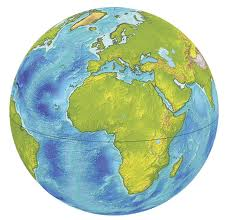
\includegraphics[scale = 0.5]{img/earth}
                \caption{Source image}
        \end{subfigure}
		\quad
        \begin{subfigure}[b]{0.3\textwidth}
                
\includegraphics[scale = 0.5]{img/earth_segment}
                \caption{Segmented image}
        \end{subfigure}
		\caption{Example of segmenting an image. In this example the number of clusters specified is 3.}
		\label{fig:segmentation}
\end{figure}

\noindent \textbf{Background subtraction} \par
Background substraction (also known as foreground detection) is a process often used to detect moving objects with a static camera. The idea is that the background remains roughly the same in every image in a video stream, while moving objects enter and leaves the stream shortly after, or become part of the background after some time have passed. The rationale is to have a background image (or reference point) and then substract the image with the new object in it. Computing the difference will result in an image with only the moving object in it, that can be used for analysis. The absolute difference is computed almost like a standard \textit{matrix substraction} as shown in Equation \ref{eq:matrix_sub}. An example of background subtraction is shown in Figure \ref{fig:background_filtering}\\

\begin{equation}
\setlength{\arraycolsep}{5pt}
 \begin{bmatrix}
  a & b \\
  c & d \\
 \end{bmatrix} - 
 \setlength{\arraycolsep}{5pt} 
 \begin{bmatrix}
  e & f \\
  g & h \\
 \end{bmatrix} =
 \setlength{\arraycolsep}{5pt} 
 \begin{bmatrix}
  abs(a-e) & abs(b-f) \\
  abs(c-g) & abs(d-h) \\
 \end{bmatrix}
 \label{eq:matrix_sub}
\end{equation}

\begin{figure}
        \centering
        \begin{subfigure}[b]{0.3\textwidth}
                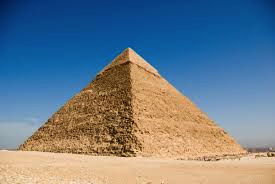
\includegraphics[scale = 0.35]{img/pyramid}
                \caption{Background image}
        \end{subfigure}
		\quad
        \begin{subfigure}[b]{0.3\textwidth}
                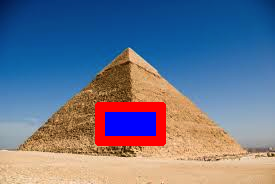
\includegraphics[scale = 0.35]{img/pyramid_new}
                \caption{Foreground image}
        \end{subfigure}
        \begin{subfigure}[b]{0.3\textwidth}
                
\includegraphics[scale = 0.35]{img/pyramid_object}
                \caption{Object detection}
        \end{subfigure}
		\caption{Example of detecting a new object on a static background. In this example all differences greater than zero is set to 255.}
		\label{fig:background_filtering}
\end{figure}

\newpage

\subsubsection{Framework} \mbox{}\par
\label{framework}
The theory behind computer vision techniques is solid. However to track an ant in an image solid theory and implementation is not enough. We have to keep in mind that this will have to be done on several consecutive images, without delaying the entire process, allowing the ant to escape the camera. Therefore effeciency is a key aspect as well. Chosing an effecient framework to help us track ants is therefore of outmost importance. OpenCV provides such a framework.\\

OpenCV is the shorthand for Open Computer Vision, and is an open source project started in 1999 and since maintained by Intel. It is written in C and C++ and runs on Linux, Windows and Mac OS X. OpenCV was designed from to beginning to be computationally efficient with a string focus on real-time applications. Another goal is to provide a simple-to-use computer vision infrastructure. Since its initial creation OpenCV has matured gradually, and along with it computer vision as well. Today OpenCV and computer vision is used in a broad context from web applications to survailance and aerial street maps.\\

Other computer vision frameworks exists but come short on several parameters. As stated in the requirements, tracking had to be done in \texttt{C}/\texttt{C++} which leaves out frameworks for higher level languages such as PyCVF for Python, imageJ for Java and OpenClooVision for C\#. Furthermore several frameworks exist that extends OpenCV or creates a simpler abstraction layer such as SimpleCV and other frameworks offers a very limited amount of features such as VisionBlocks. As a result OpenCV was chosen to be the framework of choice, both because of maturity and effeciency, but also because of the amount of computer vision features offered to its users.

\subsubsection{Realization} \mbox{}\par
Having presented several computer vision techniques and the framework used, this section will focus on applying these techniques in a real world scenario to find an actual ant within an image from a webcam. To be able to track the ant of interest and make it distinguishable from other ants, we will paint it with a color that is easier to detect than the ant itself. We want to track the ants on real ground material, and not just a static colored uniform background, and the ants available to us are either dark brown or black closely resembling the ground material found throughout Europe. It is therefore important to choose a color that is easy to detect on such material. For this reason we have chosen a white paint for testing purposes.\\

The image in Figure \ref{fig:ant} will be used as a reference point when showing how a certain computer vision technique performs in tracking the ant.

\begin{figure}[ht!]
  \centering
    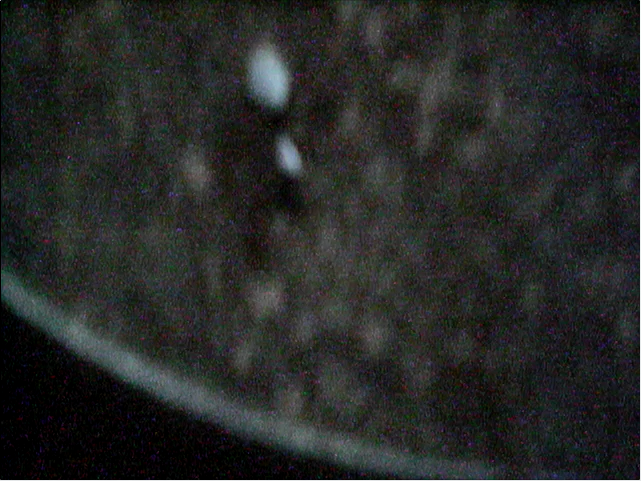
\includegraphics[scale=0.25]{img/ant.png}
  \caption{}
  \label{fig:ant}
\end{figure}

It is evident from the image in Figure \ref{fig:ant}, that the overall image is very dark. The ant itself is very hard to see, and even the white areas are dark. A way to improve this is to use the theory of \emph{Contrast and Brightness} to improve the lighting condition of the image. Figure \ref{fig:contrast_ant} shows the result of applying contrast or brightness to Figure \ref{fig:ant}. \\

\begin{figure}
        \centering
        \begin{subfigure}[b]{0.4\textwidth}
                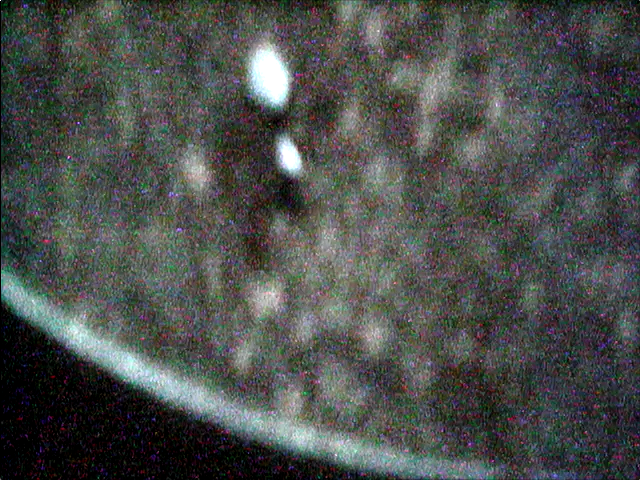
\includegraphics[scale = 0.2]{img/contrast2times}
                \caption{$\alpha = 2$}
        \end{subfigure}
		\quad
        \begin{subfigure}[b]{0.4\textwidth}
                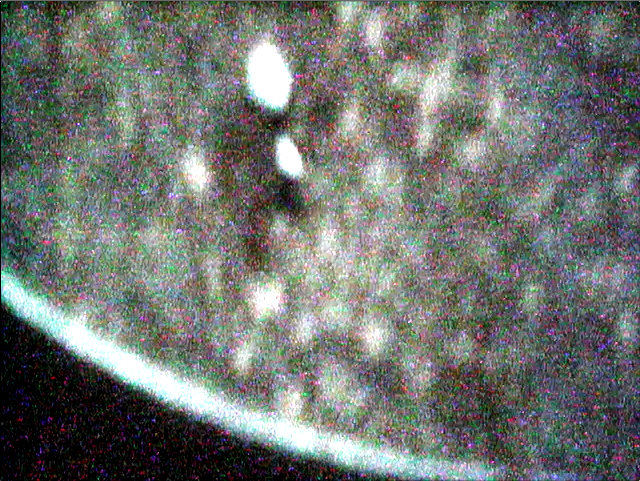
\includegraphics[scale = 0.2]{img/contrast3times}
                \caption{$\alpha = 3$}
        \end{subfigure} \hfill \\ \mbox{}\\
        \begin{subfigure}[b]{0.4\textwidth}
                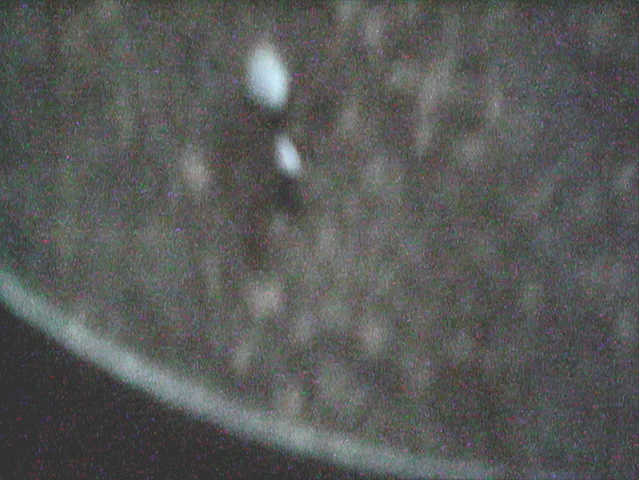
\includegraphics[scale = 0.2]{img/bright50}
                \caption{$\beta = 50$}
        \end{subfigure}
		\quad
        \begin{subfigure}[b]{0.4\textwidth}
                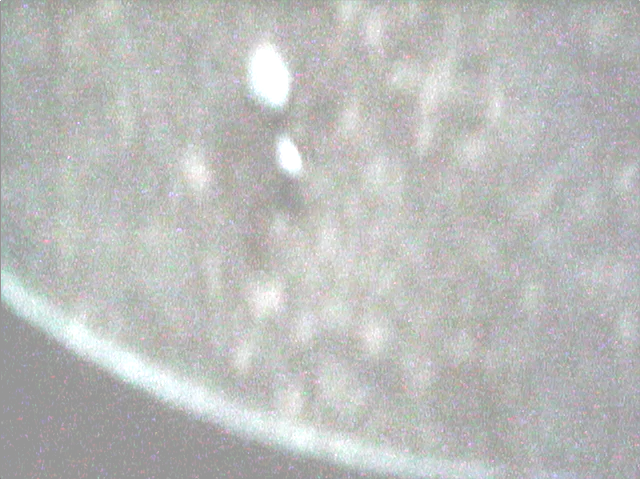
\includegraphics[scale = 0.2]{img/bright150}
                \caption{$\beta = 150$}
        \end{subfigure}
		\caption{Applying brightness or contrast to the ant image.}
		\label{fig:contrast_ant}
\end{figure}

It is clear from Figure \ref{fig:contrast_ant} that image \emph{c} and \emph{d} does not provide a proper result. Even though the image is indeed brightened, differentiating between the ant and the background has not become much easier. Small changes to the lightning condition would probably also make image \emph{d} much harder to analyse. Whether image \emph{a} or \emph{b} provides the best result comes down to what we want the most - that the object we look for is as close to clear white as possible, or that it is the most distinguishable object in the image. For colors in general, it is better for it to be distinguishable than trying to make it hit a specific color intensity. The result of image \emph{a} is therefore preferable. \\

Now that we have improved the overall quality of the image, the next task is to isolate the ant in the improved image. For this task we have three techniques available; \emph{thresholding}, \emph{image segmentation} and \emph{background subtraction}. Background subtraction have a major flaw in our case - the camera in question is in no way static. Furthermore, the area covered by the camera involves different color intensities of ground material, petri-dish edge and water. To create a background filter that would map to all these different materials, and at the same time take into consideration that they will never appear in the same part of the image, makes it almost impossible to do. In most situations there will be so many new objects in the image, that the ant might be the least changable object for every frame. This leaves us with image segmentation and thresholding.\\

Figure \ref{fig:segment_ant} shows examples of running image segmentation with different numbers of segments, \textit{K}, defined on image \emph{a} from Figure \ref{fig:contrast_ant}. It is clear from these tests that a certain number of segments are neccessary for a satisfactory result. $K=8$ and $K=10$ clearly gives the best results, however it comes at a cost; segmenting these images simply takes too much time. Even with only óne segmentation attemp for each image, it takes around one second or more to produce a result. Considering this needs to be done \emph{multiple} times within a second when using a camera, this solution is simply not feasible or possible for tracking. An ant can easily move out of a frame without the camera ever knowing, simply because it is too slow or the ant is too fast.\\

\begin{figure}
        \centering
        \begin{subfigure}[b]{0.4\textwidth}
                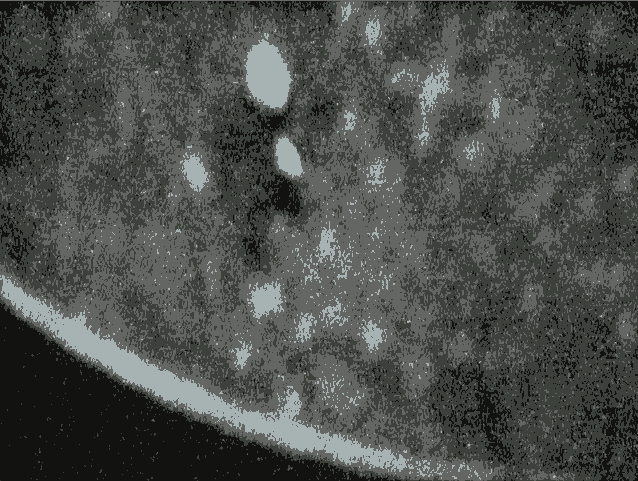
\includegraphics[scale = 0.2]{img/segment4}
                \caption{K = 4}
        \end{subfigure}
		\quad
        \begin{subfigure}[b]{0.4\textwidth}
                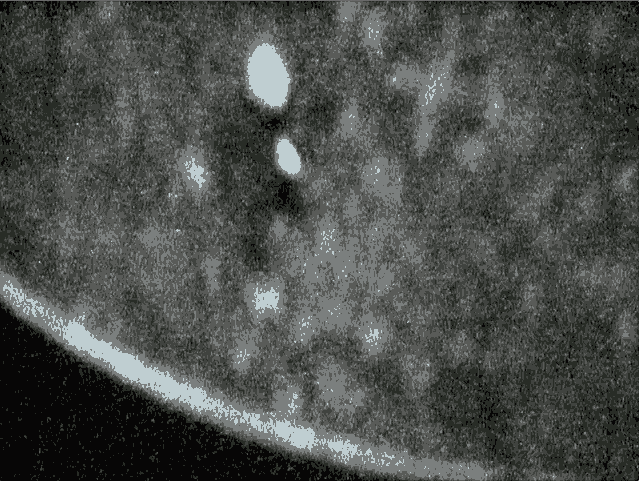
\includegraphics[scale = 0.2]{img/segment6}
                \caption{K = 6}
        \end{subfigure} \hfill \\ \mbox{}\\
        \begin{subfigure}[b]{0.4\textwidth}
                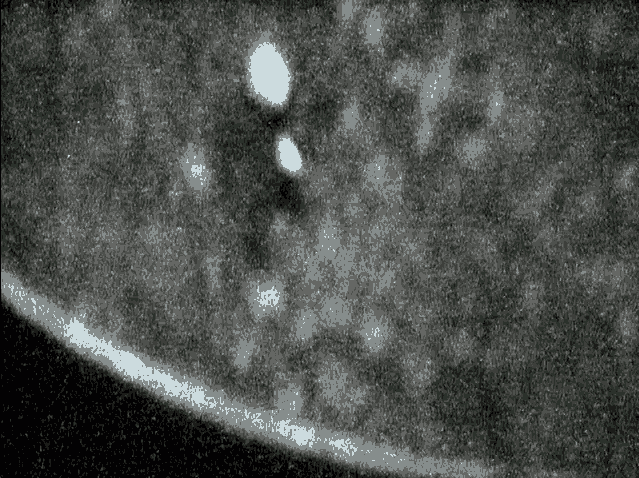
\includegraphics[scale = 0.2]{img/segment8}
                \caption{K = 8}
        \end{subfigure}
		\quad
        \begin{subfigure}[b]{0.4\textwidth}
                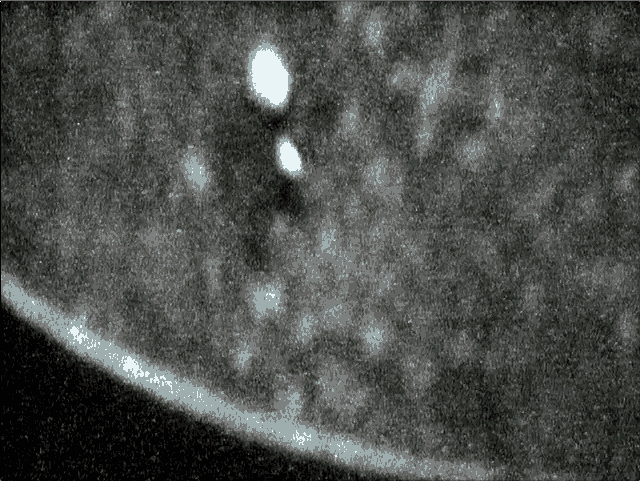
\includegraphics[scale = 0.2]{img/segment10}
                \caption{K = 10}
        \end{subfigure}
		\caption{Segmenting the ant image.}
		\label{fig:segment_ant}
\end{figure}

This leave us with only one option; thresholding. Figure \ref{fig:threshant} shows thresholding attemps on a grayscale version of image \emph{a} from Figure \ref{fig:contrast_ant}. The results of different thresholds shows us two things; firstly that image \emph{d} is a very good threshold result and secondly that we need a rather high threshold value to get this result. In contrast to segmentation, applying a threshold to our image is much faster, and usable for a steady camera stream.\\

\begin{figure}
        \centering
        \begin{subfigure}[b]{0.4\textwidth}
                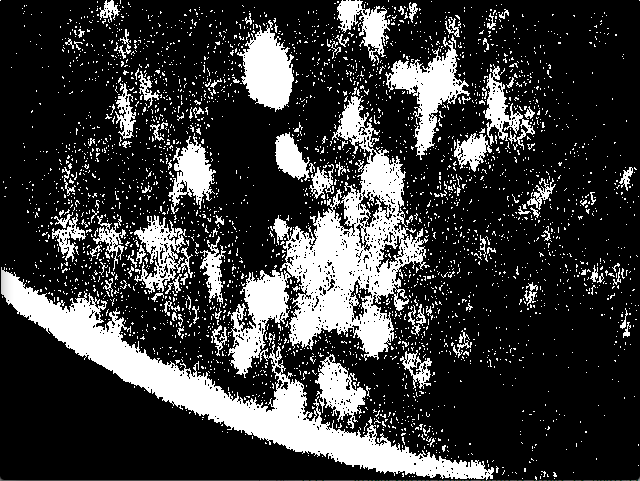
\includegraphics[scale = 0.2]{img/thresh100}
                \caption{T = 100}
        \end{subfigure}
		\quad
        \begin{subfigure}[b]{0.4\textwidth}
                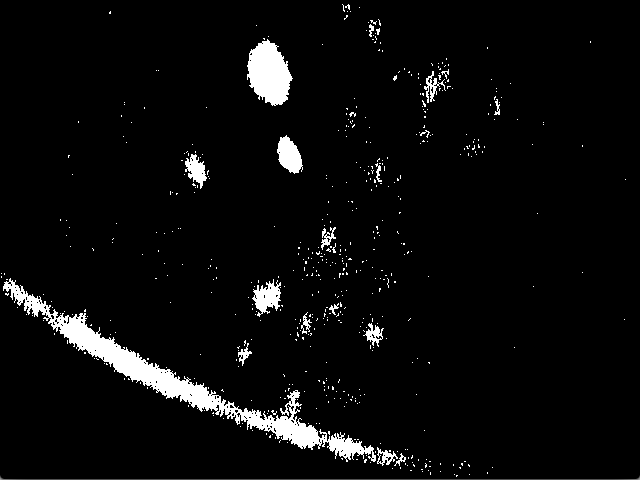
\includegraphics[scale = 0.2]{img/thresh150}
                \caption{T = 150}
        \end{subfigure} \hfill \\ \mbox{}\\
        \begin{subfigure}[b]{0.4\textwidth}
                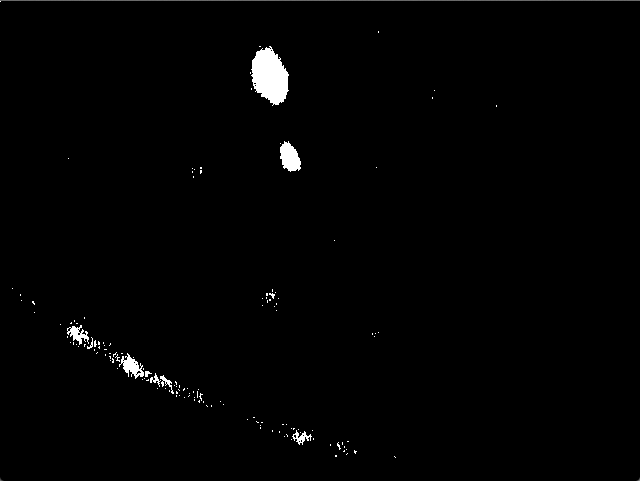
\includegraphics[scale = 0.2]{img/thresh200}
                \caption{T = 200}
        \end{subfigure}
		\quad
        \begin{subfigure}[b]{0.4\textwidth}
                
\includegraphics[scale = 0.2]{img/thresh240}
                \caption{T = 240}
        \end{subfigure}
		\caption{Thresholding the ant image.}
		\label{fig:threshant}
\end{figure}

Now that we have a satistafactory binary image that clearly shows the position of our ant, the next step is to actually get the location of the ant within the image. For this purpose we will use a \textit{blob detection}. In short, blob detection is a computer vision technique encapsulating mathematical methods that are aimed at detecting regions in a digital image. These regions differ in properties such as brightness and color from the regions surrounding it. So where segmentation seeks to partition an image, blob detection seek to find the partitions. All the pixels in a blob are considered to share similar properties.

Considering the binary image \emph{d} from Figure \ref{fig:threshant} clearly shows that we have to blobs available, that are rather large. This is of course ideal, but we might also have cases where we have smaller blobs caused by reflections on the ground or water. Therefore is is not enough to just use the first blob we find in an image - we should always use the largest blob available in the image, which hopefully, is our ant. The result of finding the largest blob in our binary image is shown in Figure \ref{fig:finalResult}.

\begin{figure}
    \captionsetup{justification=centering}
        \centering
        \begin{subfigure}[b]{0.45\textwidth}
                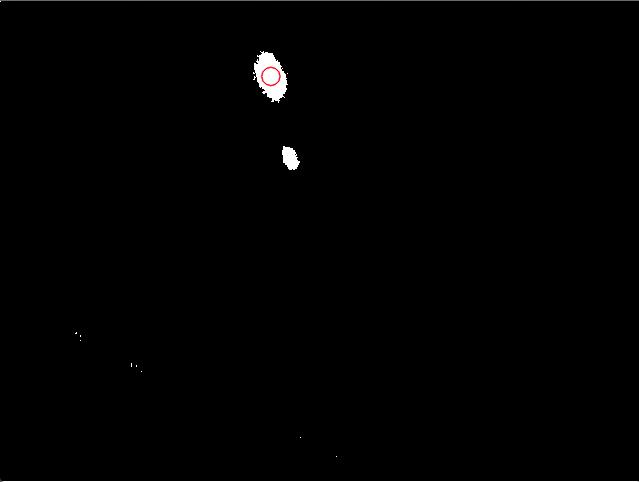
\includegraphics[scale = 0.25]{img/threshblob}
                \caption{\mbox{}\\Detected blob drawn on thresh image}
        \end{subfigure}
		\quad
        \centering
        \begin{subfigure}[b]{0.45\textwidth}
                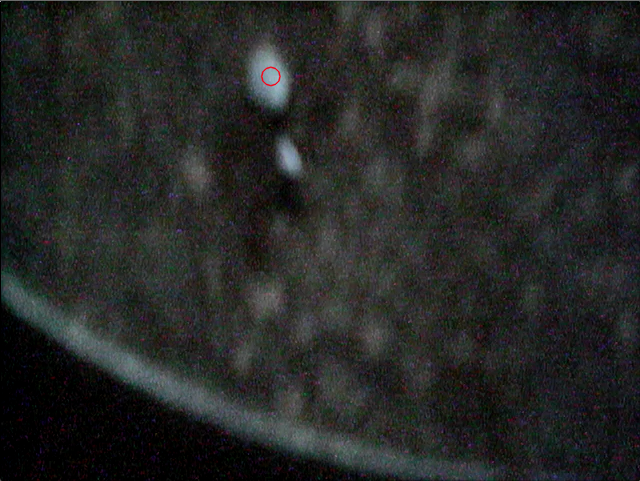
\includegraphics[scale = 0.25]{img/srcblob}
                \caption{\mbox{}\\Detected blob drawn on original image}
        \end{subfigure}
		\caption{Final result of finding the ant in our image. The detected blob is drawn on on both the thresholded image and the original ant image.}
		\label{fig:finalResult}
\end{figure}

Concluding this chapter we outline tho process of going from a raw image input to a successfully detected ant within an image, based on both the choices and experiments from this chapter. The process is as follows:

\begin{enumerate}
    \item Increase the contrast of the raw image with an alpha value of atleast 2.0.
    \item Convert the contrasted image to grayscale.
    \item Threshold the contrasted image with a threshold value of atleast 240.
    \item Run blob detection on the thresholded image.
    \item Output the largest blob from the blob detection on the original image.
\end{enumerate}

\section{Camera feedback and robot control}

%!TEX root = Report.tex

\subsection{Integration with camera}

To track the ants present in the petri dish, the plotter is equipped with two low resolution standard web cameras connected directly to the computer using USB. One of the cameras are strapped on a piece of hard plastic holding the lens face-down, thus monitoring the entire scene from a height of approximately XX cm. This camera is referred to as the overhead camera and is supposed to provide the user with the big overview, as well as a canvas to draw statistical overlays on, like heatmaps etc. The second camera is mounted directly on the plotter arm and follows the ant as it moves around in the arena. We will refer to this camera as the mobile camera.

Choosing relatively low resolution cameras has been a deliberate decision, as processing is done on a per-frame basis, meaning there is good reason to believe that a higher pixel-density would increase processing time and thus prevent the camera from keeping up with the ant. On the other hand, the resolution should be high enough for the software to be able to identify the ant and/or the painted marker on its body. Fortunately, tests have shown that the mobile camera used in this project has been close to optimal with regards to image quality.

Another performance indicator for the mobile camera is the amount of frames it is able to record per second (FPS). To be able to maintain a stable tracking process, it is a key property that the ant is present in any two consecutive frames recorded by the camera. If this property is not held, it means that the ant is ahead of the camera, and the plotter will need to initiate a special procedure to relocate the ant. The camera needs at least as many FPS as needed for this to hold. On the other hand, more frames means more processing, which is also not good, but as long as the image quality is modest, this should not be a problem. The specific camera that was used in this project has a suitable quality, but could use a higher FPS value.

On a side note, it should be noted that the plotter is not new; the internal mechanics are sensitive and will some times cause the arm to do a fast wiggle. We experienced during testing that this blurs the camera input and may introduce small blobs similar to the one representing the ant. Thus, the plotter is in danger of being biased in a wrong direction and loose track of the ant. This problem is also likely to be reduced by using a camera with a larger FPS rate.

\subsubsection{Practical information} \mbox{}\par

\subsubsection{Communication with Plotter} \mbox{}\par
Just like the two cameras, the plotter is connected to the PC through USB. The plotter provides an old-fashioned LPT parallel port interface which is connected to a printed circuit board (PCB) converting from USB to LPT. The board has a diode that will light up when signals arrive at the USB side of the board. The diode will give a constant blue light in case of an error, but will otherwise flash green. Together with a PC and an RS232 terminal like e.g. Termite, this diode is useful for troubleshooting in case something is not working when running the TERMES software. In order to establish a connection to the plotter for debugging purposes, use the connection parameters listed in table \ref{table:connparam}

\begin{table}[ht]
\centering
\renewcommand{\arraystretch}{1.1}
\setlength{\tabcolsep}{8pt}
	\begin{tabular}{ |l|l| }
  	\hline
  	\multicolumn{2}{|c|}{Connection Parameters} \\
  	\hline
  	Baud Rate & 38400 bps \\
  	Data Bits & 8 \\
  	Stop Bits & 1 \\
  	Parity & none \\
  	Flow Control & none \\
  	\hline
	\end{tabular}
	\caption{Connection Parameters}
	\label{table:connparam}
\end{table}








Hvilken plotter er det og hvilket udstyr sidder på den
Hvordan er den sat til computeren
hvad vil vi gerne have den til (nævn at det ville have været nice at have det cross platform)
hvordan gør vi dette
hvilke "services" ender vi med at udstille til resten af programmet (flyt til koordinat, current coordinate?)
Hvordan er performance? kan videoen køre i real time? hvis nej hvad betyder det for os? skal vi skippe frames?

*   0x01 = send coordinate to plotter
 *   0x01 + 2 bytes for x + 2 bytes for y (up to 10 bits) up to 0x03FF (y probably only up to 01F0)
 *   0x02 in response = sucesss
 *   0xFE in response = failure
 
\subsubsection{Moving the camera} \mbox{}\par
Now that we know how to move the plotter, how do we move the camera when the ant moves?
what about the volume of the movement sound?
what about the speed of the movement?


%!TEX root = Report.tex

\section{Graphical user interface}

TODO


\section{Testing, evaluation and conclusion}

%!TEX root = Report.tex

\section{Process}

Hvad var process planen?
Hvordan kommunikerede vi med Harvard + vejleder?
Hvordan gik det (eval)?
Havde vi nogen problemer med det? (tidsforskel, kultur forskel)
Hvilke værktøjer brugte vi?
Virkede de efter hensigten?
Hvilke kommunikations kanaler brugte vi?
Virkede de efter hensigten? ville vi gerne have haft mere eller mindre kommunikation?
Ville vi gøre noget anderledes hvis vi skulle gøre det igen/hvad har vi lært?

Vi har modtaget video først for at kunne starte før vi fik plotteren.

Halls has defined cultures as being either high-context or low-context, which states the degree to which their culture is expressed. As an example, a low-context culture will have a lot of implicit actions, where a high-context culture will act more explicitly.
- Olson, J. \& G. Surprises in Remote Software Development Teams. p. 58


%!TEX root = Report.tex

\subsection{Reflection}
In this section we will discuss and reflect upon issues that we believe have had a potential influence on the outcome of the project. These include a discussion of how the situation would have looked if we could have removed the requirement of using a mobile camera and how the project could have benefited from using a different plotter. \\

Using a mobile camera is a requirement because users would potentially like to be able to stimulate the ant using food or a pheromone stick attached to the camera. However, excluding this requirement, we have no reason to believe after this project that it should not be possible to reach the same goals using only the overhead camera. This would of course require an overhead camera with a suitable resolution and tests to verify that frames with the chosen resolution can be processed in a satisfactory amount of time. The relation between the resolution of the current cameras and processing times leads us to believe that it would indeed be possible to increase resolution without increasing the processing time to an unacceptable level. However, it requires testing to know exactly how much. \\

On the positive side, using only an overhead camera would get rid of the mechanical wiggles that cause the frames to become blurry, remove sounds that might affect the behavior of the ant and remove shadows from the mobile camera on the plotter table. Furthermore, it will increase (but not remove) the upper bound we need to put on processing time per frame as there is no mobile camera to lose track of the ant between frames. With only an overhead camera, it would even be possible to do tracking based on   video files instead of a live camera input and thus eliminate all bounds on processing time (because all frames could be recorded beforehand). \\

Ignoring reflections from the water could be a useful addition to the software. Whenever a blob would be detected, we could convert its pixel position to a camera coordinate, and based on this, measure the distance to the center of the petri dish. If the distance is greater than the radius of the petri dish the blob must be a reflection from the water and can be safely ignored. A corner case where this would fail is if the ant is close to the edge, causing the reflection to merge with the ant and create a single blob where ant and reflection is indistinguishable.\\

Reducing the sounds from the plotter is also something we could have achieved by exchanging the plotter for a different model. Choosing a different plotter would also open possibilities for choosing a better model that has smoother moving arms.

%!TEX root = Report.tex

% Overvej at kalde dette afsnit "Experimentation" eller "Testing"
% 
% vis hvornår det virker og hvornår det ikke virker. 
% Se at det virker når vi regnede med at det virkede.
% 
% Hvad tester vi?
% Hvordan tester vi det?
% Virkede det efter hensigten?
% Hvorfor/hvorfor ikke?
% Er der nok testing?
% Hvordan kan man lave mere testing?
% Er der andre måder vi kunne have testet på? (fordele og ulemper ved det)

\subsection{Testing the tracking software with real ants}

Having solved the problem of finding an ant on a single image and integrated our software with the XY-plotter and camera, this section focus on testing how the integrated solution works with a video feed of an ant running arond in a controlled environment.\\

The test were performed in a ordinary office environment, with the plotter placed on a table. The room were only litten by daylight, and we used the setup explained in section (REF HANDLING ANTS), with a petridish filled with ground material surround by water, as can be seen in Figure (INSERT FIGURE WITH IMAGE OF SETUP). According to our experimentation in (INSERT REF TO EXPERIMENTATION) we painted our ant with a white color to have the best possible color for tracking.\\

In the following we will show several results of running the software, both where the tracking works as intented, but also situations where the software does not work. We will end this section with a summary of the challenges presented by this real-time testing and suggest possible solutions to the problems and an overall evaluation of how the software together with the plotter an camera performs performs. We will also comment on the important observations done during testing.\\

We will begin by showing several images from the test where the software tracking works. Examples can be seen in Figure \ref{fig:ant_tracking}. We are showin both the final thresholded image, as well as the original image. For this test, the images were contrasted with an $\alpha = 2.0$ and $T = 240$.\\

\begin{figure}
        \centering
        \begin{subfigure}[b]{0.35\textwidth}
                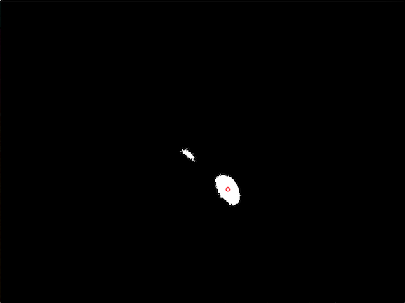
\includegraphics[scale = 0.3]{img/good1t}
                \caption{}
        \end{subfigure}
		\quad
        \begin{subfigure}[b]{0.35\textwidth}
                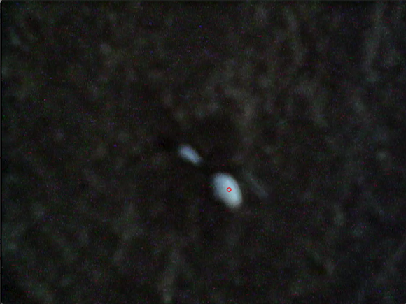
\includegraphics[scale = 0.3]{img/good1}
                \caption{}
        \end{subfigure} \hfill \\ \mbox{}\\
        \begin{subfigure}[b]{0.35\textwidth}
                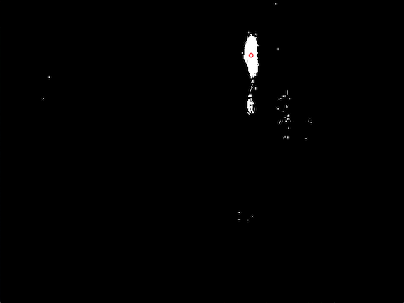
\includegraphics[scale = 0.3]{img/good2t}
                \caption{}
        \end{subfigure}
		\quad
        \begin{subfigure}[b]{0.35\textwidth}
                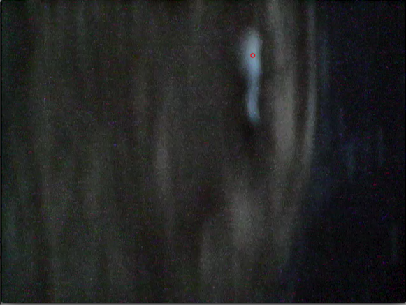
\includegraphics[scale = 0.3]{img/good2}
                \caption{}
        \end{subfigure}\hfill \\ \mbox{}\\
        \begin{subfigure}[b]{0.35\textwidth}
                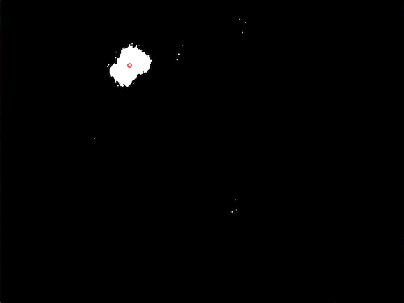
\includegraphics[scale = 0.3]{img/good3t}
                \caption{}
        \end{subfigure}
		\quad
        \begin{subfigure}[b]{0.35\textwidth}
                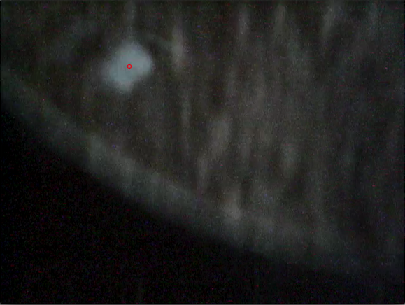
\includegraphics[scale = 0.3]{img/good3}
                \caption{}
        \end{subfigure}\\ \mbox{}\\
        \begin{subfigure}[b]{0.35\textwidth}
                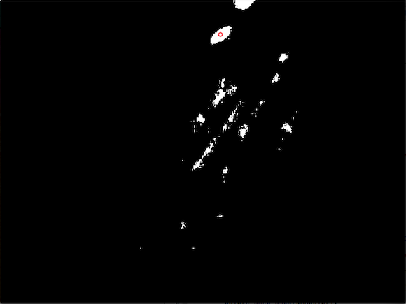
\includegraphics[scale = 0.3]{img/good4t}
                \caption{}
        \end{subfigure}
		\quad
        \begin{subfigure}[b]{0.35\textwidth}
                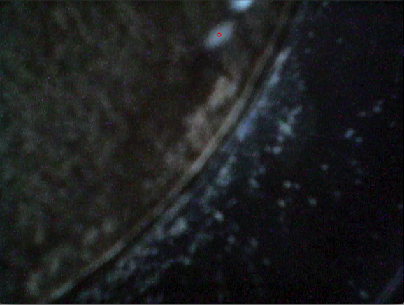
\includegraphics[scale = 0.3]{img/good4}
                \caption{}
        \end{subfigure}
		\caption{Examples of real-time ant tracking.}
		\label{fig:ant_tracking}
\end{figure}

\newpage

%!TEX root = Report.tex

\section{Threats to validity}

Høj lyd / hastighed kan skræmme myrerne til at flytte sig hurtigere/mere.
Lav resolution
Myrer =/= termitter
myrer bevæger sig ikke som i naturen
temperatur + luftfugtighed + vind + lys osv.
Masser af genskær (lysforhold)
TODO

\subsection{Threats to internal validity}
Internal Validity is concerned with confirming that the correlation between the treatment and the outcome is indeed casual, and not accidental, or caused by some third variable that has not been observed. For example we may discover that all programmers in C were faster than programmers in Java, but forget that all the programmers in Java took the experiment very late at night, when they were tired.

\subsection{Threats to external validity}
External validity discusses how far the results are generalizable, or in other words how representative the sample of subjects and the circumstances of the experiment were, to be able to draw general conclusion. Do you expect the same results to be confirmed in somewhat modified conditions?


%!TEX root = Report.tex

\subsection{Related Work}

\noindent \textbf{TERMES: An Autonomous Robotic System for Three-Dimensional Collective Construction} \par

Paper by Kirstin Petersen, Radhika Nagpal and Justin Werfel \cite{termes1}. This paper presents a hardware system and high-level control scheme for autonomous construction of 3D structures. The hardware system consist of mobile autonomous robots and a collection of passive marked blocks. The general idea is to use swarm robotics to enable efficient construction even in extraterratial or disaster areas. The behavior of the robots is much like ants and termites in thaat sensing is entirely onbaord and each robot acts indenpendently of each other. Our contribution to the field can help enhance this project in the long run through analysis of the collaboration patterns of natures own swarms: ants and termites. By analysing how termites build their large hives one could potentially find a great way for swarm robots to collaborate when building structures.

http://www.eecs.harvard.edu/ssr/papers/iros11wksp-werfel.pdf




%!TEX root = Report.tex

\subsection{Future Work}
%More statistics
%Bias mode
%Support for multiple plotters
%Plotter control as a library
%Tests with real termites
%Developer terminal/log (print was is sent to the plotter and the answer + the hard tracking coordinate data)
%Color pickers i GUI

Because time was a limited resource for our team there were features we did not implement and ideas for additional functionality that could have been included. This section describes a short list of the possible extensions to the project we might have worked towards, were we given more time. \\

The first task would be to implement the optional requirements listed in Section \ref{requirements}. While some of these requirements are relatively easy to implement, given the right amount of time, some of them are more challenging. For example tracking multiple ants can be difficult unless all ants are marked, however this is something the current solution cannot solve. \\

When all optional requirements were fulfilled it could be beneficial to support multiple types of XY-plotters. The plotter we used was a little dated and being able to switch to another XY-plotter could be very practical. Of course this would also imply testing with a number of different plotters to see whether or not the same result could be reproduced. To support multiple plotters one could implement plotter control as an external API to make it easy for other applications to control the plotter. \\

One of things we really wanted to do, but did not have the opportunity to, was to test with real termites. The solution was designed to be able to switch between different insects of different sizes and to test with real termites would be a strong indicator of how well this switch would work. \\

%!TEX root = Report.tex

\subsection{Conclusion}

TODO


%!TEX root = Report.tex

\section{Defition of terms}
TODO


\begin{thebibliography}{9}
    
		\bibitem{termite} Thiadmer Riemersma. (2013, December 2). \textit{Termite: a simple RS232 terminal} [Online]. Available: \url{http://www.compuphase.com/software_termite.htm}
        
        \bibitem{opencv} Itseez. (2013, December 2). \textit{OpenCV} [Online]. Available: \url{http://opencv.org/}
        
        \bibitem{fogn} Rune Larsen. (2013, December 2). \textit{Kæmpemyrer (Campotonus ligniperdus)} [Online]. Available: \url{http://www.fugleognatur.dk/artsbeskrivelse.asp?ArtsID=8063}
        
        \bibitem{github} Nikolaj Aaes. (2013, December 2). \textit{Aaes/TermiteTracker} [Online]. Available: \url{https://github.com/Aaes/TermiteTracker}
        
		\bibitem{halls} J. \& G. Olson. (2013, December 2). \textit{Surprises in Remote Software Development Teams from lectures} [Online]. Available: \url{http://dl.acm.org/citation.cfm?id=966804}
        
        \bibitem{termes1} Kirstin Petersen, Radhika Nagpal and Justin Werfel. (2013, December 2) \textit{TERMES: An Autonomous Robotic System for Three-Dimensional Collective Construction} [Online]. Available: \url{http://www.eecs.harvard.edu/ssr/papers/rss11-petersen.pdf}
        
        \bibitem {termes2} Kirstin Petersen, Radhika Nagpal and Justin Werfel. (2013, December 2) \textit{Distributed Multi-Robot Algorithms for the TERMES 3D Collective Construction System} [Online]. Available: \url{http://www.eecs.harvard.edu/ssr/papers/iros11wksp-werfel.pdf}
        
\end{thebibliography}

%!TEX root = Report.tex

\appendix
\section{First Appendix}

\end{document}
